
Die Informatik umfasst eine Vielzahl unterschiedlicher Fachgebiete mit teils stark variierenden Schwerpunkten. 
Dazu zählen unter anderem die Web- und Anwendungsentwicklung sowie der Bereich der IT-Sicherheit und viele weitere Disziplinen. 
Im Rahmen dieser Arbeit liegt der Fokus auf dem speziellen Teilbereich der Embedded-Softwareentwicklung.

In diesem Kapitel werden die grundlegenden fachlichen und technischen Konzepte vermittelt, die zum Verständnis der weiteren Inhalte erforderlich sind.
% Ablauf des Kapitels
Zu Beginn wird eine Einführung in das Themenfeld der Embedded-Systeme gegeben, um ein klares Verständnis dafür zu schaffen, welche Unterschiede diesen Bereich kennzeichnen und wie er sich von anderen Teilgebieten der Informatik unterscheidet.
Darauffolgend werden zentrale Begriffe und Konzepte erläutert, die in der Embedded-Entwicklung eine signifikante Rolle spielen, wie beispielsweise Register, Ports, Peripherieansteuerung und hardwarenahe Programmierung.
Darüber hinaus wird technisches Hintergrundwissen vermittelt, das für das Verständnis der späteren Implementierungsschritte und der Architekturentscheidungen von Relevanz ist.

%Das Ziel dieses Kapitels besteht darin, eine solide Wissensbasis zu schaffen, auf der die Analyse bestehender Lösungen sowie die Entwicklung einer eigenen Treiber-API aufbauen können.

\section{Eingebettete Systeme}
Bevor auf die Entwicklung eingebetteter Systeme eingegangen werden kann, ist zunächst zu klären, worum es sich bei diesen Systemen handelt.
Der Begriff \emph{Embedded System} (deutsch: eingebettetes System) bezeichnet ein Computersystem, das aus Hardware und Software besteht und fest in einen übergeordneten technischen Kontext integriert ist. 
Typischerweise handelt es sich dabei um Maschinen, Geräte oder Anlagen, in denen das eingebettete System spezifische Steuerungs-, Regelungs- oder Datenverarbeitungsaufgaben übernimmt.
Ein wesentliches Merkmal eingebetteter Systeme besteht darin, dass sie nicht als eigenständige Recheneinheiten agieren, sondern als integraler Bestandteil eines übergeordneten Gesamtsystems dienen.
In der Regel operieren sie im Hintergrund und sind nicht direkt mit den Benutzern verbunden. In einigen Fällen erfolgt die Interaktion automatisch, in anderen durch Eingaben des Nutzers.

\paragraph{Definition:}
Ein Embedded System ist ein spezialisiertes, in sich geschlossenes Computersystem, das für eine klar definierte Aufgabe innerhalb eines übergeordneten technischen Systems konzipiert wurde.

\vspace{6 mm}

Die Entwicklung von Software für eingebettete Systeme ist mit besonderen Anforderungen verbunden, die sich signifikant von denen unterscheiden, die etwa in der Web- oder Anwendungsentwicklung üblich sind.
Es ist von besonderer Bedeutung, hardwarenahe Aspekte zu berücksichtigen, da die Software unmittelbar mit der zugrunde liegenden Mikrocontroller-Hardware interagiert.
Ein zentraler Aspekt dabei ist die Integration geeigneter Treiber für die jeweilige Mikrocontroller-Architektur.
Die betreffenden Treiber beinhalten Funktionen, welche den Zugriff auf die Hardware mittels sogenannter Register erlauben.
Register sind spezifische Speicherbereiche innerhalb des Mikrocontrollers, welche eine unmittelbare Manipulation des Hardware-Verhaltens ermöglichen.
Durch das gezielte Setzen oder Auslesen einzelner Bits in diesen Registern ist es möglich, beispielsweise Sensorwerte zu erfassen (z. B. das Drücken eines Tasters) oder Ausgaben zu erzeugen (z. B. das Anzeigen eines Textes auf einem Display).



\section{Begriffe und Erklärungen}

\subsection*{Microprozessor Unit (MPU)}
Ein Mikroprozessor ist ein vollständig auf einem einzigen integrierten Schaltkreis (Chip) realisierter Prozessor.
Der Prozessor ist die zentrale Recheneinheit eines Computersystems.
Seine Funktion umfasst die Ausführung von Befehlen sowie die Steuerung des Datenflusses innerhalb des Systems. 
Ein Mikroprozessor beinhaltet in der Regel Komponenten wie das Rechenwerk (\gls{alu}), Register, Steuerwerk und gegebenenfalls Zwischenspeicher (Caches), jedoch keine Peripheriefunktionen wie Speicher oder Schnittstellen. 
Diese müssen extern angebunden werden.
Der Begriff "Mikrocomputer" wird verwendet, um ein auf Basis eines Mikroprozessors aufgebautes Gesamtsystem zu definieren. 
Derartige Systeme sind in klassischen PCs, Laptops oder Servern häufig anzutreffen.
In diesen Geräten wird der Mikroprozessor mit externem RAM, ROM, I/O-Komponenten und weiteren Funktionseinheiten kombiniert.

Demgegenüber ist der Mikrocontroller für spezifische Steuerungsaufgaben mit integrierten Peripheriefunktionen konzipiert. 
Der Mikroprozessor findet dagegen meist in leistungsfähigen, aber nicht auf eine konkrete Aufgabe spezialisierten Systemen Anwendung. 
Insbesondere für allgemeine Rechenaufgaben, komplexe Betriebssysteme sowie Anwendungen mit hohem Ressourcenbedarf erweist sich dieser Prozessor als geeignet.

\subsection*{Microcontroller Unit (MCU)}
Ein Mikrocontroller ist ein vollständig auf einem einzigen Chip realisierter Mikrocomputer, der neben dem eigentlichen Prozessor (CPU) auch sämtliche für den Betrieb notwendigen Komponenten integriert. 
Zu den Komponenten eines solchen Systems zählen in der Regel Programmspeicher (Flash), Datenspeicher (\gls{ram}), digitale Ein- und Ausgänge (\gls{gpio}), Timer, Kommunikationsschnittstellen (wie \gls{uart}, \gls{spi}, \gls{i2c}, \gls{can}) sowie in vielen Fällen analoge Peripheriekomponenten wie Analog/Digital-Wandler oder Pulsweitenmodulation-Einheiten.

Mikrocontroller werden für spezifische Steuerungs- und Regelungsaufgaben konzipiert und finden typischerweise Anwendung in eingebetteten Systemen, wie beispielsweise Haushaltsgeräten, Fahrzeugsteuerungen, Industrieanlagen oder IoT-Geräten. 
Die Geräte zeichnen sich durch einen geringen Energieverbrauch, eine kompakte Bauform, niedrige Kosten und eine direkte Hardwareansteuerung aus. 
Im Vergleich zu Mikroprozessoren sind für den Grundbetrieb von Mikrocontrollern keine externen Komponenten erforderlich, was besonders kompakte und zuverlässige Systemlösungen ermöglicht.


%\subsection*{Hardware Architektur}
%- CISC vs. RISC
%
%- Cortex Familie


\subsection*{Register}
Register sind kleine, besonders schnell zugängliche Speicherzellen, die direkt im Prozessor untergebracht sind. 
Im Gegensatz zu anderen Speicherformen, wie etwa RAM oder Flash, zeichnen sich Register durch extrem kurze Zugriffszeiten aus. 
Dies ist darauf zurückzuführen, dass sie Teil des zentralen Rechenwerks sind. 
Die Nähe zur Recheneinheit ist dabei von entscheidender Bedeutung, insbesondere für grundlegende Operationen wie das Zwischenspeichern von Werten, Adressen oder Zustandsinformationen während der Programmausführung.

Im Kontext eingebetteter Systeme und insbesondere bei der Treiberentwicklung spielen sogenannte speicherabbildende Register (Memory-Mapped Registers) eine zentrale Rolle. 
Diese sind Teil der Hardwareperipherie (wie \gls{gpio}, \gls{spi} oder \gls{uart}) und über spezifische Speicheradressen ansprechbar. 
Durch das Schreiben in oder Lesen aus solchen Registern können spezifische Hardwarefunktionen aktiviert, deaktiviert oder abgefragt werden.

Ein konkretes Beispiel ist ein \gls{gpio}-Ausgangsregister: Wird ein bestimmtes Bit darin gesetzt, liegt am zugeordneten Pin ein logisches High-Signal an. 
Die exakte Kenntnis über die Position und Signifikanz dieser Bits ist essenziell für die direkte Hardwareprogrammierung und die korrekte Umsetzung von Treibern.
\\
Register werden somit nicht nur für die interne Funktionsweise des Prozessors relevant, sondern bilden auch die Schnittstelle zwischen Software und Hardware. Es sei darauf hingewiesen, dass diese Elemente die Konfiguration, Steuerung und das Auslesen externer Peripheriekomponenten ermöglichen und somit das zentrale Element bei der Low-Level-Programmierung darstellen.

\subsection*{Peripherie}
Unter dem Begriff der \emph{Peripherie} versteht man im Kontext der Embedded-Softwareentwicklung sämtliche Ein- und Ausgabeschnittstellen, die eine Interaktion des Mikrocontrollers mit seiner Umwelt ermöglichen.
Peripheriegeräte stellen die Verbindung zwischen der digitalen Rechenlogik des Mikrokontrollers und der realen Welt her.
Sie ermöglichen die Erfassung, Verarbeitung und Ausgabe physikalischer Signale wie Temperatur, Licht oder der Betätigung eines Tasters.
Ein moderner Mikrocontroller, wie etwa ein STM32, ist bereits mit einer Vielzahl an integrierten Peripherieeinheiten ausgestattet, darunter digitale Ein-/Ausgänge (GPIOs), serielle Kommunikationsschnittstellen (UART, SPI, I2C, CAN), analoge Wandler (ADC, DAC), Timer oder PWM-Module. 
Die als \emph{On-Chip} bezeichneten Komponenten sind integraler Bestandteil des Mikrocontrollers und können über zugehörige Register programmiert und gesteuert werden.
Zusätzlich zur integrierten Peripherie besteht die Möglichkeit, über die physischen Pins des Mikrocontrollers auch externe Peripheriegeräte anzuschließen. 
Die Verbindung erfolgt in der Regel mittels Steckverbindungen, wie etwa Jumper-Kabeln, Steckbrücken, Pin-Headern oder speziellen Anschlussleisten auf Entwicklungsboards. 
In der Regel werden zu diesem Zweck Steckbretter (Breadboards) oder Lochrasterplatinen verwendet, um eine übersichtliche und flexible Verdrahtung zu gewährleisten. 
Externe Bauteile, wie etwa Sensoren (Temperatursensor), Aktoren (LED), Displays oder Speicherbausteine, werden über gängige Schnittstellen wie I2C, SPI, UART oder digitale GPIOs mit dem Mikrocontroller verbunden.
Die Kommunikation mit externen Geräten wird durch die Peripheriemodule des Mikrocontrollers realisiert. 
Für den zuverlässigen Betrieb sind in der Regel spezifische Softwaretreiber erforderlich, die die Initialisierung, Datenübertragung und gegebenenfalls die Fehlerbehandlung übernehmen.

% TODO: chap4 Peripherie: Parallel/Seriell; synchron/asynchron; für alle nochmal drüber gehen
\subsubsection*{General Purpose Input Output}
Der Begriff \emph{General Purpose Input/Output} (GPIO) bezeichnet universelle digitale Ein- und Ausgänge, die sich durch eine hohe Flexibilität für verschiedenste Aufgaben auszeichnen.
Sie ermöglichen es dem Mikrocontroller zum Beispiel, digitale Signale zu lesen (Input) oder zu erzeugen (Output), um etwa Taster auszuwerten oder LEDs anzusteuern. 
GPIOs stellen somit die einfachste Form der Peripherieanbindung dar.

\subsubsection*{Serial Peripheral Interface}
Die Schnittstellen des \emph{Serial Peripheral Interface} (SPI) ist ein synchrones, serielles Kommunikationsprotokoll, das insbesondere für die schnelle und effiziente Datenübertragung über kurze Distanz zwischen einem Master- und einem oder mehreren Slave-Geräten eingesetzt wird. 
Die primäre Aufgabe des Protokolls besteht in der Verbindung von \gls{mcu}s mit integrierten oder externen Komponenten, zu denen unteranderem  Sensoren, Speicher, Aktoren sowie Displays zählen.
SPI arbeitet synchron, d.h. Sender und Empfänger teilen sich ein gemeinsames Taktsignal.
Der Master ist derjenige, der diesen Takt vorgibt und bereitgestellt.
Dadurch wird eine präzise, zeit-sensitive Übertragung ermöglicht. 
Die zentrale Eigenschaft von \gls{spi}, die das gleichzeitige Senden und Empfangen ermöglicht ist die Unterstützung der Voll-Duplex-Kommunikation.
% TODO: SPI: Quellenverweise einfügen.
Der \gls{spi}-Bus verwendet meistens vier physikalische Leitungen:
\begin{itemize}
	\item \gls{miso} / \gls{cipo} für die Kommunikation vom Master zu den Peripheriegeräten (Slaves).
	\item \gls{mosi} / \gls{copi} für die Kommunikation von den Peripheriegeräten zum Master.
	\item \gls{ss} / \gls{cs} für die Auswahl des gewünschten Peripheriegerätes.
	\item \gls{sclk} als Taktleitung, die den vom Master vorgegebenen Takt enthält.
\end{itemize}

In der Regel dient der Mikrokontroller als Master, der den Datenfluss steuert.
Mittels des Slave-Signals ist es der \gls{mcu} möglich, gezielt Slaves anzusprechen.
Dabei ist darauf zu achten, dass jeweils nur ein Slave die Kommunikation aktiv durchführen darf, um eine Kollision auf Bus zu vermeiden.

\gls{spi} zeichnet sich im Vergleich zu anderen seriellen Protokollen wie \gls{i2c} durch eine vereinfachte Implementierung und eine deutlich höhere Datenübertragungsrate aus. 
Allerdings fehlen eine standardisierte Adressierung und Fehlerprüfung, was den Einsatz auf kurze Distanzen und überschaubare Topologien begrenzt. 


\subsubsection*{Universal Asynchronous Receiver Transmitter}
Der \emph{Universal Asynchronous Receiver Transmitter} (UART) ist ein asynchrones Kommunikationsprotokoll, das insbesondere für die serielle, asynchrone Punkt-zu-Punkt-Kommunikation zwischen zwei Geräten eingesetzt wird. 
Das Protokoll eignet sich für verschiedene Anwendungsbereiche, darunter als Debugging-Schnittstelle, der Kommunikation von Sensoren, GPS-Modulen sowie die Kommunikation mit Computern über USB-zu-Seriell-Wandler. 
Im Gegensatz zu synchronen Schnittstellen wie SPI ist für UART kein gemeinsames Taktsignal erforderlich.
Die Datenübertragung passiert hier asynchron über zwei Leitungen: eine für das Senden (Transmitter TX) und eine für das Empfangen (Receiver RX).
Die Synchronisation basiert auf einer zuvor festgelegten Baudrate (Bits pro Sekunde), die von beiden Geräten unabhängig voneinander eingehalten werden muss.
Die Kommunikation, d.h. die Datenübertragung erfolgt in sogenannten Frames. Ein typisches \gls{uart}-Frame besteht aus:
% TODO: UART: Quellenverweise einfügen
\begin{itemize}
	\item \textbf{Startbit}, das den Begin eines Datenframes signalisiert,
	\item \textbf{Datenframe}, bestehend aus fünf bis acht Bits,
	\item \textbf{Paritätsbit}, das einer einfacheren Fehlererkennung dient und
	\item \textbf{Stopbit}, das das Ende des Datenframes markiert.
\end{itemize}

In Abhängigkeit von der Implementierung unterstützt UART Simplex-, Halbduplex- und Vollduplex-Kommunikation. 
In einer Vielzahl von Mikrocontrollern ist UART als Hardwaremodul integriert, wodurch die serielle Kommunikation effizient und mit minimalem Softwareaufwand realisiert werden kann. 
Dennoch erfordert die korrekte Konfiguration – insbesondere die Wahl der Baudrate, des Paritätsmodus und der Anzahl von Stoppbits – besondere Sorgfalt, da Abweichungen zu Datenverlust oder Kommunikationsfehlern führen können.
Ein weiterer Vorteil von UART ist seine Einfachheit in Aufbau und Handhabung: Es werden lediglich zwei Leitungen benötigt. 
Die Kommunikation ist prinzipiell auf zwei Geräte beschränkt (Punkt-zu-Punkt-Verbindung), da UART keine native Unterstützung für Bussysteme mit mehreren Teilnehmern bietet.

\subsubsection*{Controller Area Network}
Das \emph{Controller Area Network} (CAN) ist ein robustes, asynchrones Bussystem, das insbesondere in der Automobilindustrie eine weite Verbreitung findet. 
Es ermöglicht eine zuverlässige Kommunikation zwischen mehreren Steuergeräten (Nodes), auch unter schwierigen elektromagnetischen Bedingungen. 
Der Einsatz von CAN in sicherheitskritischen Anwendungen beruht auf zwei wesentlichen Eigenschaften: 
\begin{itemize}
	\item der prioritätsbasierten Arbitrierung
	\item der integrierten Fehlererkennung
\end{itemize}
 
 Diese Eigenschaften gewährleisten eine hohe Ausfallsicherheit.

\subsection*{Common Microcontroller Software Interface Standard (CMSIS)}
Der \emph{Common Microcontroller Software Interface Standard} stellt einen von Arm entwickelten Industriestandard dar, der eine einheitliche Softwarearchitektur für Mikrocontroller auf Basis der Arm-Cortex-Prozessorfamilie bereitstellt.
Der Begriff "CMSIS"  bezeichnet eine Sammlung von Schnittstellen, Softwarekomponenten, Header-Dateien, Entwicklungswerkzeugen und Workflows.
 Die Sammlung soll die Portabilität, Wiederverwendbarkeit und Effizienz im Bereich der Softwareentwicklung für eingebettete Systeme steigern.
Das Ziel von CMSIS besteht darin, eine konsistente und herstellerübergreifende Abstraktion der zugrunde liegenden Hardware bereitzustellen, um die Integration verschiedener Entwicklungswerkzeuge und Bibliotheken zu erleichtern.
Die Standardisierung ermöglicht es Entwicklerinnen und Entwicklern, auf einheitliche Weise auf Prozessorfunktionen, Peripherie und Betriebssystemfunktionen zuzugreifen, unabhängig vom konkreten Mikrocontrollerhersteller.

Die Sammlung ist in mehrere Module unterteilt, darunter:
\begin{itemize}
	\item \textbf{CMSIS-Core:} Definieret standardisierter Zugriffsmöglichkeiten auf CPU-Register und Systemfunktionen sowie auf Start- und Systeminitialisierungscode.
	\item \textbf{CMSIS-Driver:} Definiert eine einheitliche Schnittstelle für Peripherietreiber wie UART, SPI oder I$^2$C.
	\item \textbf{CMSIS-DSP:} Stellt eine optimierte Lösung für die digitale Signalverarbeitung bereit und unterstützt sowohl Vektor- als auch Matrizenoperationen.
	\item \textbf{CMSIS-RTOS:} Stellt eine standardisierte API für Echtzeitbetriebssysteme zur Verfügung, um portierbare RTOS-Anwendungen zu ermöglichen.
	\item \textbf{CMSIS-Pack:} Fungiert als Infrastruktur, die der Bereitstellung und Verwaltung von Softwarepaketen sowie der Verwaltung von Gerätedaten in Entwicklungsumgebungen dient.
\end{itemize}

Damit bildet CMSIS die Grundlage einer Vielzahl von Entwicklungsumgebungen, wie beispielsweise Keil MDK, STM32CubeIDE oder CMSIS-kompatibler CMake-basierter.


\subsection*{Toolchain}
Der Begriff "Toolchain" bezeichnet eine Sammlung von aufeinander abgestimmten Softwarewerkzeugen, die gemeinsam zur Übersetzung, Verlinkung und Bereitstellung von lauffähiger Software auf einem Zielsystem verwendet werden. 
Insbesondere in der Entwicklung von Embedded Systems spielt die Toolchain eine entscheidende Rolle im Entwicklungsprozess, da sie die Verbindung zwischen der Hochsprachenprogrammierung und der spezifischen Hardwareumgebung herstellt.

Zu den typischen Bestandteilen einer Toolchain gehören:
\begin{itemize}
	\item Compiler
	\item Assembler
	\item Linker
	\item Debugger
\end{itemize}

Zusätzlich kommen im Prozess Hilfswerkzeuge wie Make- oder CMake-System, Flash-Tools und Binärkonverter zum Einsatz.
In der Entwicklung von Mikrocontrollern findet in der Regel der Einsatz sogenannter Cross-Toolchains statt, die auf einem Host-System ausgeführt werden (beispielsweise Windows oder Linux). 
Diese erzeugen Code für eine andere Zielarchitektur, wie beispielsweise einen Arm-Cortex-M-Prozessor. 
Ein verbreitetes Beispiel ist die GNU Arm Embedded Toolchain, die aus den Komponenten \texttt{arm-none-eabi-gcc}, \texttt{arm-none-eabi-ld}, \texttt{arm-none-eabi-gdb} und weiteren Elementen besteht.

%\subsection*{Compiler/Cross-Compiler}
%Bei einem \emph{Compiler} handelt es sich um Werkzeug der Softwareentwicklung, das Quellcode, der in einer Hochsprache wie C oder C++ verfasst wurde, in Maschinencode übersetzt. 
%Dieser kann direkt vom Zielprozessor ausgeführt werden. Im Gegensatz zur Ausführung durch einen Interpreter, welcher den Code zur Laufzeit Zeile für Zeile ausführt, erfolgt beim Kompilieren eine vollständige Übersetzung des Codes vor der Ausführung des Programms.
%
%Im Bereich der Embedded-Systems-Entwicklung finden häufig sogenannte Cross-Compiler Anwendung, da die Software typischerweise auf einem anderen System (Host) entwickelt wird als jenem, auf dem sie später ausgeführt wird (Target).
%Ein bekanntes Beispiel ist GCC (GNU Compiler Collection), das in Toolchains wie \texttt{arm-none-eabi-gcc} zum Einsatz kommt.
%Neben der reinen Übersetzung ermöglichen sie auch statische Codeanalysen, Optimierungen hinsichtlich Laufzeit oder Speicherbedarf und tragen damit maßgeblich zur Qualität eingebetteter Software bei.



\subsection*{CMake}
CMake ist ein plattformübergreifendes Open-Source-Werkzeug zur Automatisierung des Buildprozesses in der Softwareentwicklung
Der sogenannte Metabuild-Generator (\autoref{fig:cmake_generators}) dient als eine Art universeller Konfigurator, der mithilfe Konfigurationsdateien, den \texttt{CMakeLists.txt}-Dateien, spezifische Build-Systeme für eine Vielzahl unterschiedlicher Plattformen und Entwicklungsumgebungen generiert.
Unter diesen Build-Systemen finden sich beispielsweise Makefiles für Unix/Linux, Projektdateien für Visual Studio oder Xcode.

\begin{figure}[H]
	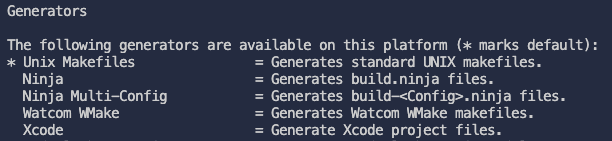
\includegraphics[width=\textwidth]{cmake_generators.png}
	\caption{Ausschnitt einer Liste von verfügbaren Generatoren.}
	\label{fig:cmake_generators}
\end{figure}

Ein wesentlicher Vorteil von CMake liegt in der Trennung von Quell- und Build-Verzeichnissen, was sogenannte Out-of-Source-Builds ermöglicht.
Diese Vorgehensweise trägt zur Schaffung einer übersichtlichen Projektstruktur bei und vereinfacht die Verwaltung von Build-Artefakten.
Zusätlich fördert CMake die hierarchische Strukturierung von Projekten mittels der Implementierung von modularen CMakeLists.txt-Dateien in Unterverzeichnissen.
Dieser Ansatz steigert die Wartbarkeit und Skalierbarkeit komplexer Softwareprojekte.

\subsection*{Make und Makefiles}
Make ist ein traditionelles Werkzeug zur Automatisierung von Build-Prozessen, das sogenannte Makefiles zur Steuerung dieser Prozesse einsetzt.
Die Makefiles definieren Regeln, mit deren Hilfe der Quellcode, abhängig davon ob sich etwas im Code geändert hat, kompiliert und verlinkt wird.
Make findet für gewöhnlich Anwendung in der direkten Steuerung von Kompilierungsprozessen.
 Es besteht jedoch auch die Möglichkeit, es zur Steuerung anderer Build-Systeme einzusetzen.
In einigen Projekten findet ein manuelles Makefile Verwendung, welches ausschließlich CMake mit spezifischen Parametern aufruft, um den eigentlichen Build-Prozess zu initialisieren.
In einem solchen Szenario fungiert Make als Wrapper über CMake und ersetzt nicht dessen eigentliche Build-Logik.


% TODO: chap4 Hintergrundwissen: Embedded Kontext; Software-Architektur Kontext; ...
\section{Hintergrundwissen}
Die Entwicklung eingebetteter Systeme erfordert ein grundlegendes Verständnis sowohl der Hardwarearchitektur als auch der zugrunde liegenden Softwarewerkzeuge.
Der zentrale Baustein solcher Systeme ist der Mikrocontroller, der typischerweise aus einem Prozessor, Speicher und integrierten Peripherieeinheiten, wie beispielsweise GPIO, UART, SPI oder CAN, aufgebaut ist.
Die Ansteuerung dieser Peripherie erfolgt durch Register, auf die über definierte Adressen zugegriffen werden kann.
Der unmittelbare Zugriff auf Register findet in der Regel in Maschinensprache oder Assemblersprache statt;
je größer und komplexere Projekte werden, desto schwieriger wird die Wartung und Portierbarkeit.
Aus diesem Grund werden Hochsprachen wie C oder C++ eingesetzt, die eine abstraktere, strukturierte Programmierung ermöglichen. 
Die Übersetzung dieser Hochsprachen in den erforderlichen Maschinencode erfolgt mittels eines Compilers, der anschließend vom Prozessor ausgeführt werden kann.
Für die genannte Zielarchitektur, z.B. auf einem ARM-Mikrocontroller, werden sogenannte Cross-Compiler eingesetzt, da die Zielarchitektur von der Entwicklungsplattform, z.B. PC, abweichen kann.
Ein wesentlicher Bestandteil der Toolchain ist in der Regel ein Assembler, ein Linker sowie ein Debugger.




























